\documentclass[jou,12pt,a4paper]{apa6}

%%%%%%%%%%%%%%%%%%%% Loading packages %%%%%%%%%%%%%%%%%%%% 
\usepackage{csquotes}
\usepackage[american]{babel}
\usepackage{amsmath, amssymb, graphicx,gensymb}
\usepackage{fixltx2e} % Misc Latex fixes
\usepackage{url}
\usepackage{threeparttable}
\usepackage[capposition=top]{floatrow}
\usepackage[colorlinks=true,citecolor=blue]{hyperref}
\usepackage{apacite}

%%%%%%%%%%%%%%%%%%%% Set some paramters %%%%%%%%%%%%%%%%%%
\setlength{\parindent}{10mm}
\setlength{\parskip}{0mm}
\graphicspath{ {Figures/} } % path to images

%%%%%%%%%%%%%%%%%%%% Title and such %%%%%%%%%%%%%%%%%%%%%%
\title{\LARGE Investigating dimensionality of globally distributed functional brain networks}
\shorttitle{Dimensionality of functional neural networks}

\author{Lukas Snoek}
\affiliation{University of Amsterdam}
\authornote{Lukas Snoek, student nr. 10126228, University of Amsterdam, Email: lukassnoek@gmail.nl.}

%%%%%%%%%%%%%%%%%%%%%%%%%%%%%%%%%%%%%%%%%%%%%%%%%%%%%%%%%
%  OPTIONAL STUFF  									
%	\leftheader{Snoek}		ONLY IN [jou] MODE			
%	\journal{Journal of Awesomeness}					
%	\volume{2(3)}										
%	\note{version 1}									
%%%%%%%%%%%%%%%%%%%%%%%%%%%%%%%%%%%%%%%%%%%%%%%%%%%%%%%%%

\abstract{In the past decade, cognitive neuroscience witnessed a paradigm shift from functional localization to distributed representations of psychological processes in the brain. In studies using functional MRI, multivariate analyses have been a popular choice to investigate these distributed representations. In the psychological literature, however, the term ``distributeness'' has been used ambiguously and inconsistently, as multivariate representations may be present locally within cortical areas or globally across the entire brain. While local and global multivariate representations are likely encoded at different levels of organisation (across voxels versus across brain areas, respectively), most multivariate analyses are performed without taking the representation's multivariate dimensionality into account. This study investigates the dimensionality of large-scale functional networks involved in representing emotional experience, which is hypothesized to be encoded over brain regions. Several dimension-reduction strategies are performed on an existing dataset containing globally distributed networks representing components of emotional experience. It is shown that multivariate classification accuracy is maintained, or even improved, following up to a dimensionality reduction as drastic as factor 1000 relative to standard univariate feature selection methods. Given these results, recommendations are outlined for maximizing potential of multivariate analyses of globally distributed functional networks in cognitive neuroscience.}

%%%%%%%%%%%%%%%%%%%% Begin doc! %%%%%%%%%%%%%%%%%%%%
\begin{document}

%%%%%%%%%%%%%%%%%%%% Titlepage! %%%%%%%%%%%%%%%%%%%%

\begin{titlepage}

\newcommand{\HRule}{\rule{\linewidth}{0.5mm}} 
\center 

% Headings
\textsc{\LARGE Graduate School of Psychology}\\[1cm] 
\textsc{\Large University of Amsterdam}\\[1cm]

% Title section
\HRule \\[0.4cm]
{ \huge Research Master's Psychology - MSc. Thesis}\\[0.4cm] 
\HRule \\[1.5cm]
 
% Author section & version/data info
\begin{minipage}{0.4\textwidth}
\begin{flushleft} \large
\emph{Author:}\\
Lukas \textsc{Snoek} 
\end{flushleft}
\end{minipage}
~
\begin{minipage}{0.4\textwidth}
\begin{flushright} \large
\emph{Supervision:} \\
\textsc{Dr. H.S. Scholte} 
\end{flushright}
\end{minipage}\\[1cm]

% Logo

\includegraphics[width=60mm]{uva_logo_inv}\\[1cm] 

% Data
{\large \today}\\[2cm]

\vfill 

\end{titlepage}

%%%%%%%%%%%%%%%%%%%% Start article %%%%%%%%%%%%%%%%%%%%

\maketitle

\section{INTRODUCTION}
A key question in the field of cognitive neuroscience is how the brain represents information. A traditional approach in the neuroimaging community is to investigate the representations of psychological concepts and processes as significant activations or deactivations of parts of the brain using functional magnetic resonance imaging (fMRI). This type of analysis is commonly referred to as ``univariate analysis'', because they test assess each unit of measurement (i.e. voxels) in the brain separately as independent univariate models \cite{friston1994}. Often, studies utilizing such a univariate approach yield color-rendered brain-maps with significant (de)activations, leading researchers to conclude that the plotted regions (or ``blobs'') are involved in the psychological concept or process under examination. 

In the past two decades, univariate analyses have been used to localize psychological concepts and functions to particular brain areas. Results were often interpreted as finding a neural correlate or mapping for the particular psychological concept or process under examination. Implicitly, researchers implicitly engaged in a type of ``neo-phrenology'' in which unique function-structure mappings are pursued \cite{poldrack2010}. Examples of brain regions that have emerged within this framework are the the amygdala, which has gradually become known as the ``fear processing area'' \cite{ledoux2003} and the lateral fusiform gyrus, which has become the ``face processing area'' (and was, in fact, named the \emph{fusiform face area}).  

In the light of our current understanding of the organization of the human brain, these function-structure mappings are unwarranted. At present, several counter-examples have been put forward for every purportedly selective function-structure mapping \cite{poldrack2010}. The amygdala has, for instance, been implicated in processing stimulus novelty \cite{blackford2010} and the fusiform face area has, for instance, been associated more generally with processing highly familiar objects \cite{tarr2000}. These counter-examples suggest that univariate analyses map more basic, domain-general psychological processes underlying the investigated concept instead of its representational content.

In the early 21st century, the cognitive neuroscience community gradually moved from this functional localization perspective to a more ``multivariate'' perspective \cite{sporns2002,barrett2013}. Instead of studying \emph{which} regions (de)activate during a particular psychological process, neuroscientists started to investigate \emph{how} brain areas or a network of brain areas encode and represent this particular process. Rather than treating individual voxels as independent sources of information, researchers realized that by modeling psychological concepts and processes as multivariate representations consisting of interdependent voxels, they could investigate how the brain represents, instead of responds to, information.

One of the first studies to show that the human brain encodes psychological concepts as distributed, multivariate representations was described in the seminal paper by \cite{haxby2001}. They showed that different object categories are represented in a distributed fashion across the ventral visual cortex. Importantly, they demonstrated that object categories could be distinguished from each other when controlling for potential mean activation differences, which formed the basis of the widespread perspective that MVPA capitalizes on information above and beyond mean activation levels. Their approach, for which they used the term Multivariate Pattern Analysis (MVPA), gained popularity quickly as it appeared to provide a more sensitive analysis as opposed to univariate analyses \cite{jimura2012} and was consistent with and complemented the emerging network-oriented theoretical framework \cite{bressler2010}. Several new types of multivariate analyses were developed in the succeeding years, including the successful application of machine learning classifiers to distinguish neural representations (e.g. \citeNP{cox2003}) and representational similarity analyses to characterize relations between neural patterns in a continuous, rather than discrete, manner \cite{kriegeskorte2008}. 

Currently, MVPA analyses are widespread in almost all domains of cognitive, affective, and social neuroscience. For example, in vision research, MVPA has been applied to correctly decode stimulus orientation in subregions of V1 \cite{kamitani2005}. At a coarser scale, researchers have shown that it is possible to decode episodic memory traces across the human hippocampus \cite{chadwick2010}. More recently, MVPA has surfaced in the social and affective neuroscience literature, in which it has been used to investigate broadly distributed representations of social and emotional processes. For example, \citeA{kassam2013} has shown that MVPA can be used to decode representations of different emotions. 

MVPA thus seems to be applicable to various levels of representational content. It is not unlikely, however, that the way representations are manifested in the brain differ depending on whether one investigates, for example, low-level stimulus features such as spatial frequency versus high-level cognitive or affective processes such as decision-making or emotional experience. Despite this, it appears that many ``high-level'' MVPA-studies adopt analysis standards and parameters which are common in ``low-level'' MVPA studies. As will be argued next, this conformity to analysis standards of low-level multivariate analyses leads to implicit, and potentially invalid, assumptions about the spatial scale and dimensionality of representations.

\subsection{Assumptions of spatial scale}
In the early years of MVPA, the technique was mainly used in cognitive neuroscience studies investigating low-level psychological concepts such as the representation of basic stimulus features (e.g. orientation, color, and motion) and object category. These low-level representations are known to be represented in spatially-restricted, contiguous patches of cortex, such as the representation of low-level stimulus features in (extra)striate cortex \cite{kamitani2005,parkes2009} and the representation of object categories in ventral temporal cortex \cite{haxby2001,eger2008}. With the application of MVPA to higher-level psychological concepts and processes, the assumption of locality of spatial scale seems to have remained largely unchanged. This assumption is, however, inconsistent with the emerging perspective of cognitive processes and higher-level psychological concepts as interacting, global brain networks \cite{bressler2010,barrett2013}. Despite this, many MVPA studies on these higher-level topics have restricted their analyses to a spatially-restricted, contiguous subset of the brain. 

One possible explanation for the tendency to restrict multivariate analyses to small, spatially-contiguous subsets of the brain is the need for stringent dimensionality reduction in multivariate analyses. Typical MVPA datasets usually suffer from what is known as the \emph{curse of dimensionality} \cite{haynes2015}, which is defined within machine learning as having more features (i.e. voxels) than samples (i.e. trials), which leads to serious problems in terms of overfitting. (Overfitting, here, is a term used to describe low generalizability of the fitted model to new, independent data, due to spurious modelling of noisy characteristics of the data). With state-of-the-art MRI-scanners, patterns of functional activation may amount to 250,000 voxels per trial, while typical experiments contain often not more than 100 stimulus presentations per condition. Therefore, MVPA studies often must perform a type of \emph{feature selection} (also known as dimension reduction) in order to reduce the feature-to-sample ration. 

Commonly, feature selection methods reduce dimensionality by limiting the spatial scale at which representations are investigated, which essentially limit or even preclude the possibility of revealing globally distributed representations. For example, one prevalent MVPA technique, the \emph{multivariate searchlight} \cite{kriegeskorte2006}, maps representations by analyzing representations in small spherical clusters of voxels throughout the brain (see for example \citeNP{clithero2009}). Although it is theoretically possible to extend the radius of the sphere to accommodate larger clusters, in practice most searchlights contain not more than 100 voxels. Moreover, although searchlights are often applied across the entire brain to reveal possibly multiple \emph{independent} sites at which the representation is encoded, searchlight analysis does not allow to investigate representations as a \emph{dependent} set of spatially-segregated clusters. 

Another common technique that reduces features by limiting the spatial extent of neural representations is \emph{region-of-interest analysis} (ROI-analysis; \citeNP{norman2006}), in which the representational space is reduced to a single brain area (see for example \citeNP{chavez2015,harry2013}). Here, an example would be to investigate representations of negative versus neutral emotions solely in the amygdala (see e.g. \citeNP{martinez2014}. Like searchlight analyses, representations could be investigated across several regions-of-interest (by for example investigating the insula and orbitofrontal cortex in addition to only the amygdala), but this does again assume that representations are independently encoded in these regions and cannot investigate whether representations are encoded in a set of dependent, spatially-segregated regions.

One way to reduce the effects of the curse of dimensionality and at the same time remain the possibility of revealing global representations is to adopt fully data-driven feature selection on the entire set of voxels. A popular whole-brain feature selection method is to select only the voxels with the largest univariate differences across conditions (usually referred to as \emph{univariate feature selection}; \citeNP{mitchell2004}). In other words, per voxel, a t-test (or ANOVA in case of more than two conditions) is computed to investigate univariate condition differences and only voxels with an f-statistic above a certain threshold are selected. Another whole-brain feature selection method is to select the most ``stable'' voxels across stimuli presentations of the same condition (see e.g. \citeNP{shinkareva2008,baucom2012}, which is operationalized as selecting voxels with the highest mean correlation among pairwise correlations across stimulus repetitions within the same experimental condition.          

A major advantage of these whole-brain feature selection methods is that they are, a priori, blind to spatial scale of the selected voxels and therefore allow for investigation of globally distributed representations. This technique is therefore especially useful in analyzing widespread functional networks, which are often reported in studies on higher-level cognitive processes. Recently, several MVPA studies on higher-level psychological concepts and processes have shown that, indeed, whole-brain feature selection yields representations consisting of various spatially-discontinuous clusters. \citeA{kassam2013}, for example, used whole-brain stability-driven feature selection to reveal a broadly distributed network involved in representation of discrete emotions, including regions from the frontal lobe (orbitofrontal cortex), temporal lobe (anterior temporal lobe), and parietal lobe (supramarginal gyrus). Similarly, studies on other high-level psychological concepts and processes, including example Theory of Mind \cite{corradi2014}, motivation \cite{etzel2015}, and emotional valence \cite{baucom2012}, reveal globally-distributed representations across the brain. 

(Theoretically, instead of univariate feature selection, one could use multivariate feature selection methods (such as Recursive Feature Elimination) to select sets of voxels. However, doing this at a whole-brain level is computationally near impossible, as this would entail testing all possible combinations of 250,000 voxels. Therefore, this technique is most often used after other dimensionality techniques haven been applied, such as region-of-interest selection \cite{norman2006}. Moreover, dimension reduction techniques involving linear transformation of features into components, such as PCA, are another possible who-brain feature selection method, but are rarely used in fMRI research and therefore not discussed.)

\subsection{Assumptions of dimensionality}
Given that high-level representations are encoded in clusters of voxels across the brain, it remains unclear what the dimensionality of these representations entails. Currently, most MVPA analyses, regardless of the representation's spatial scale, implicitly assume that representational information is encoded across voxels, meaning that each voxel within a representation carries unique information. Several MVPA studies have argued that multivariate analyses provide unique information about representations in terms of fine-grained patterns of voxel activity, above and beyond any potential univariate difference that might exist between conditions \cite{mur2009,kriegeskorte2006}. The landmark MVPA study by \citeA{haxby2001}, for instance, demonstrated that the study's measured representational patterns did not depend on univariate differences across conditions, as the classification accuracy was not affected by removing the voxels with the largest univariate amplitudes from the representations. In a similar vein, some MVPA studies control for univariate influences by subtracting the mean activation from the investigated representation (i.e. demeaning) to be able to conclude that resulting analysis results are truly driven by \emph{multidimensional} information instead of \emph{unidimensional} univariate influences (e.g. \citeNP{harrison2009,larocque2013, misaki2010}).  

While there is indeed some evidence for truly multivariate representations for low-level stimulus features in visual cortex (e.g. \citeNP{kamitani2005,parkes2009} and object category in ventral visual cortex (e.g. \citeNP{haxby2001,eger2008}), little is known about the dimensionality of more global representations often found in studies on higher-level psychological concepts and processes. Several lines of research suggest that with increases in ``globality'' of representations, information from individual voxels becomes less important. In other words, in global representations, information is likely encoded across informational units \emph{larger} than voxels and the representation's dimensionality is likely lower than the amount of voxels involved.

\begin{figure*}[ht]
\floatfoot{\textbf{Figure 1}: Three basic types of representations, which vary in spatial distribution (local versus global) and level of encoding (univariate, implying uniformity/redundancy between spatially clustered voxels, versus multivariate, implying encoding of unique information across voxels). Strictly speaking, all patterns are multivariate, but the level of encoding here refers to dimensionality of clusters within global representations.}
\centering
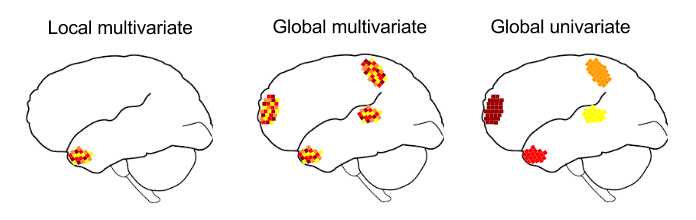
\includegraphics[scale=.55]{spatialDist2}
\end{figure*}

The study by \citeA{brants2011} directly tested this hypothesis by examining the effect of spatial smoothing on voxel patterns within the ventral visual cortex. They showed that spatial smoothing removes information about low-level stimulus features (in this case, spatial frequency) but leaves higher-level category information intact, suggesting different spatial scales for representations of different types of information (see \citeNP{drucker2009} for an example at an even lower spatial scale). Another line of evidence comes from the observation that many MVPA studies in social and affective neuroscience find representations of globally distributed \emph{clusters} of voxels (e.g. \citeNP{oosterwijk2015,kassam2013,corradi2014}). This clustering is unlikely if individual voxels within these clusters carry unique information. This dependence between voxels within clusters has been further supported by the fact that spatial smoothing \cite{oosterwijk2015,kassam2013} does not affect information encoded within representations encoded across clusters. These studies show that spatially-clustered voxels are highly correlated and thus, individually, carry redundant information about the representation. Essentially, the dimensionality of the representations is thus as high as the amount of uncorrelated informational units, whether these are voxels or clusters.  

In sum, the literature on multivariate representations of psychological concepts and processes suggest that three types of representations may exist, which are differentiated by their spatial scale and dimensionality. Low-level stimulus features and, at a slightly coarser scale, object category appear to be ``local multivariate'' (i.e. locally represented with voxels as independent informational units). Higher-level psychological concepts and processes, such as emotions, motivation, and decision-making, appear to be represented globally as spatially discontiguous clusters. Moreover, as spatial scale increases, voxels seem group in highly correlated clusters, implying that clusters instead of voxels encode independent sources of representational information. The question remains untested whether global representations are ``global multivariate'', implying voxel-level information, or ``global univariate'', in which mean activity within clusters contains the information which truly makes up the representation. This question about the dimensionality of global representations forms this study's main research question. 

\subsection{Current study}
To investigate the dimensionality of global representations, this study reanalyses the data from a previous study (\citeNP{oosterwijk2015}; see appendix A for a justification of the deviation from the original proposed experiment). In this study, we examined the neural overlap between components of self-experienced emotions and understanding emotions in others using multivariate pattern analysis with a linear support vector machine classifier \cite{chang2011}. Here, we reanalyse the data from only the self-experienced emotion patterns, because this data yielded the largest effect size (60\% classification accuracy at 33.3\% chance level) and the most robust global representation (see figure 2). Note that the observed global representation in the \citeNP{oosterwijk2015} study appears to correspond to global representations of emotion networks in several other MVPA studies \cite{kassam2013,saarimaki2015,kragel2015} and univariate studies (see for a meta-analysis \citeNP{lindquist2015}).

\begin{figure*}[ht]
\floatfoot{\textbf{Figure 2}: Global representation of self-experienced emotion components in the \citeNP{oosterwijk2015} study. The representation reflects the univariate feature selection as normalized difference scores across conditions averaged over iterations and subjects. Difference scores are computed as the average pairwise differences between the mean patterns of conditions, normalized across voxels. The global representation contains several spatially-segregated clusters, including clusters in the anterior temporal lobe, lateral occipital complex, supramarginal gyrus/angular gyrus (temporal-parietal junction), inferior frontal gyrus, frontal pole (dorsolateral prefrontal cortex), and central opercular cortex.} 
\centering
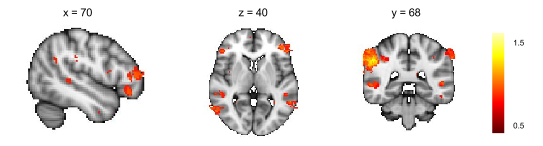
\includegraphics[width=\textwidth,height=5cm]{UnivariateFeatureSelection}
\end{figure*}

Given the apparent spatial dependence between voxels in highly correlated clusters, we hypothesize that, instead of multivariate patterns across voxels, mean activity within clusters encompasses the true dimensionality of global representations. If this is indeed the case, the set of averaged clusters should contain the same representational information as the same data in which no within-cluster averaging has been performed. To investigate this hypothesis, we analyzed the data in three different ways. First, as a benchmark, we performed univariate feature selection before classification, effectively disregarding the possible lower dimensionality of the data ('original analysis'). Second, as a proof of concept, we averaged features within a set of predefined regions-of-interest, spanning the entire gray matter volume, and subsequently performed a classification analysis with this set of averaged brain regions as features ('ROI-average analysis'). Third, as a more sensitive follow-up on the proof-of-concept, we perform a cluster-correction procedure on the selection of voxels yielded by an initial univariate feature selection. Clusters resulting from this cluster-correction procedure are subsequently averaged and used as features in the classification analysis ('cluster-average analysis'; see figure 3 for a graphical representation of these two analyses). 

We expect that, if representational information is indeed encoded in spatially-correlated clusters, above-chance classification is still possible in the ROI-average analysis and classification accuracy in the cluster-average analysis is the same as or improved with respect to the original analysis.

\begin{figure*}[ht]
\floatfoot{\textbf{Figure 3}: Graphical representation of the two performed analyses. The 'ROI-average analysis' (upper diagram) averages features within regions from a whole-brain parcellation and uses these ROI-averages as features. The 'cluster-average analysis' performs a cluster-correction procedure on the features yielded by an initial univariate feature selection and subsequently uses the within-cluster averages as features.} 
\centering
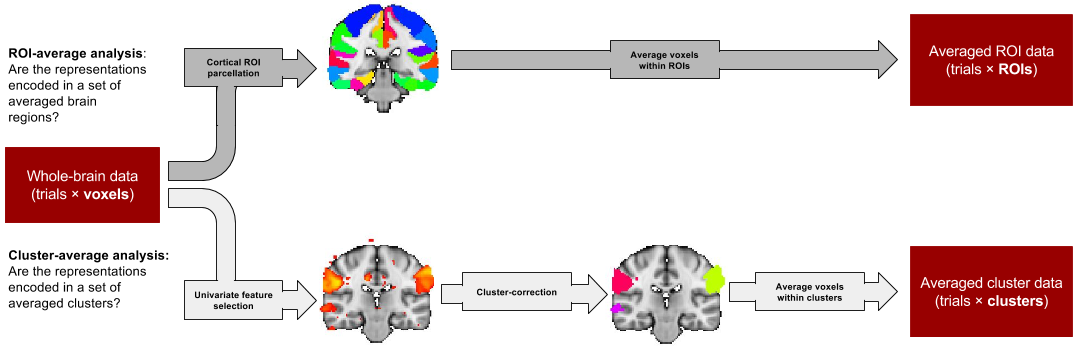
\includegraphics[width=\textwidth,height=8.5cm]{methods}
\end{figure*}

\section{METHODS}

\subsection{Dataset}
The dataset used for this research is from the \citeNP{oosterwijk2015} study. The goal of this study was to examine the neural overlap between representations of \emph{self}-focused emotional experience and representations of processes involved in understanding emotions of \emph{others}. Specifically, the study hypothesized that the same basic psychological processes -- representations of (1) sensorimotor, (2) interoceptive, and (3) situational information -- underlie both emotion experience in the self and emotion understanding of others. Using a multivariate classifier, it was shown that these representations of these three components in the self could be reliably decoded from their respective neural patterns and, importantly, that these neural representations of self-focused emotion components could be used to differentiate the corresponding components involved in emotion understanding of others significantly above chance (for a more nuanced interpretation of the results, see the original article).

This study only reanalyses data from the self-focused emotional imagery task. In total, 12 subjects completed two identical runs of this task. The stimuli consisted of short linguistic cues describing either emotional actions or expressions (representing the sensorimotor component; n = 20), bodily feelings (representing the interoception component; n = 20), or situations (representing the situational component; n = 20). Examples would be, for example, ``To make a fist'', ``To have a racing heart'', and ``Your house is on fire'', respectively. Participants were asked to imagine these actions, expressions, feelings, and situations as if they were experiencing those themselves. The stimuli (120 in total; 20 per condition, two runs) were presented in a fully event-related design for six seconds each, with a fixed inter-stimulus-interval of two seconds. Fucntional MRI data was acquired using a 3T Philips Achieva MRI-scanner, using echo-planar-imaging with a TR of 2000 ms and a TS of ... (for more details on the experimental materials, design, and scan parameters, see \citeNP{oosterwijk2015}).

\subsection{Preprocessing and first-level analysis}
The functional data from the two runs were preprocessed using various FSL functions. Preprocessing steps included slice-time correction, motion correction, spatial smoothing (FMWH: 5 mm), temporal filtering (Savitsky-Golay filter), and registration to subject-specific anatomical T1 images and subsequently to standard MNI152 (2mm) space using a non-linear transform. Resulting preprocessed timeseries were subjected to a first-level (subject-level) GLM. Single-trial regressors were created by convolving trial-specific stimulus onsets with a canonical HRF, modelled using a double gamma function. Beta-coefficients yielded by the GLM were standardized by their variance, effectively yielding patterns of t-values per trial. After masking these patterns by a gray matter mask (excluding white matter and CSF voxels) derived from the Harvard-Oxford probabilistic cortical atlas in FSL (without a minimum probabilistic threshold), subject-specific matrices of voxels (269102) $\times$ trials (120) were created to be used in the classification analysis.    

\section{RESULTS}

\subsection{Benchmark analysis}
As a benchmark analysis, a classification analysis with the same parameters as the \citeNP{oosterwijk2015} study was performed. Due to the switch from analysis environment in MATLAB to a Python/Numpy environment, reported results in this benchmark analysis may differ slightly from the results reported in \citeNP{oosterwijk2015}.

\subsubsection{Analysis set-up and parameters}
The initial parameter values for this benchmark analysis were chosen in the \citeNP{oosterwijk2015} study through a procedure resembling hyperparameter optimization through grid-search. In total, thirteen subjects were tested across two identical experimental sessions, of which the data was partitioned into two independent sets, counter-balanced across sessions. On one set, the `optimization-set', various analysis parameters were tested to achieve the best possible classification accuracy. Tested parameters included spatial smoothing kernels (from 0 mm to 10 mm FWHM), low-pass filters (from 0 to 2 seconds), the use of independent component analysis (ICA) for data cleanup, different maskers for for feature indexing (whole brain vs. various separate ROIs), the amount of test-trials per cross-validation run (from 1 to 5), and the lower bound for voxels' differentiation scores during univariate feature selection. The best performing parameter set (FHWM of 5mm, no low-pass filter, no ICA, whole-brain gray matter mask, 4 test-trials, and a lower bound of 2.3 for differentiation scores) was subsequently cross-validation on the remaining `validation set'. 

\subsubsection{Benchmark results}
- average/std of amount of features
- classification score
- 
 
\subsection{ROI-average analysis}
As proof of concept ...

\subsubsection{Analysis set-up and parameters}

\subsubsection{ROI-average results}

\subsection{Cluster-average analysis}

\subsubsection{Analysis set-up and parameters}

\subsubsection{Cluster-average results}

\subsection{Interim conclusions}

\subsection{A note on demeaning to prove dimensionality}

\subsection{Redundancy in global representations}




\section{DISCUSSION}

Future directions:
grid-search of cluster-min/zval, specified to individuals to account for ideosynchracy

\subsection{What are we measuring: Representations or processes?}

\bibliographystyle{apacite}
\bibliography{refs}

\newpage
\onecolumn
\vspace*{1px}
\section{\Huge \textnormal{Appendix}}
\vspace{25px}
\subsection{\LARGE \textnormal{Appendix A: Justification of deviation from proposal}}
\vspace{10px}

\noindent As originally described in the Research Master Thesis Proposal, we planned to use a new, custom-made experimental paradigm to manipulate the development of valence-associations using a emotion-laden narrative. After the run in which stimuli were condition through the narrative, a run would follow in which the conditioned-stimuli would be shown in isolation to assess the developed valence-associations ('post-test'). To test the strength of the valence-associations, classification accuracy between the neural, positive, and negative stimuli was proposed. It was hypothesized that successful classification (i.e. significantly above chance level) would be based upon a global functional network representing affective valence, akin to previous univariate findings (see the meta-analysis by \citeNP{lindquist2015}). 

Initially, a pilot study was done with two participants, both experienced as participating in fMRI research but unfamiliar with the research question or hypotheses. For both participants, the full experimental protocol was executed. As discussed with the project's supervisor, Dr. H.S. Scholte, the project would only be continued if the two pilot subjects would show a significant main effect in the post-test, operationalized as a classification accuracy above chance. Note that multivariate classification analyses, such as used in this scenario, are performed within subjects.   

Unfortunately, classification accuracy of valence (neutral vs. positive vs. negative) was below chance for both subjects, for both the character-stimuli, the location-stimuli, as well as valence-pooling across character and location-stimuli. This null-finding implies that the narrative failed to condition the stimuli with valence. To exclude the possibility that below-chance accuracy was caused by a possible bias in the feature selection method, multiple alternative feature selection strategies were assessed (ROI-based, whole-brain univariate feature selection with different cut-offs scores). Again, no significant effect was observed in any of the ROIs, regardless of feature selection method. Moreover, as a control analysis, it was assessed whether character-stimuli could be distinguished from the location-stimuli using our classifier, which should be possible given the consistent and robust visual dissimilarity between these conditions. Indeed, classifier performance in this control analysis was consistently above 95\% correct, ruling out software bugs or other analysis artifacts as causes for the analysis' null-result.

Considering the substantial costs associated with fMRI research (approximately 350 euros/hour) and limited time to finish this thesis research, we decided to discontinue the data acquisition using the proposed experimental paradigm. To check out the materials (Presentation script, narrative, images) created for the experimental paradigm, they can be downloaded from \url{https://github.com/lukassnoek/MSc_thesis/tree/master/Stimulus_delivery}.

\newpage
\vspace*{1px}
\subsection{\LARGE \textnormal{Appendix B: Post-hoc power-analysis}}
\vspace{10px}


\end{document}
